\documentclass[a4paper,twoside]{article}

\usepackage{epsfig}
\usepackage{subfigure}
\usepackage{calc}
\usepackage{amssymb}
\usepackage{amstext}
\usepackage{amsmath}
\usepackage{amsthm}
\usepackage{multicol}
\usepackage{pslatex}
\usepackage{apalike}
\usepackage{SciTePress}

%\subfigtopskip=0pt
%\subfigcapskip=0pt
%\subfigbottomskip=0pt

\begin{document}
	
	\title{\uppercase{...}}
	
	\author{\authorname{Herval Bernice Nganya Nana\sup{1}}
		\affiliation{\sup{1}Fachbereich Informatik und Medien, Technische Hochschule Brandenburg, Deutschland}
		\email{nganyana@th-brandenburg.de}
	}
	
	\keywords{...}
	
	\abstract{...}{...}
	
	\onecolumn \maketitle \normalsize \vfill
	
	\section{\uppercase{Prototyp}}
	
	In diesem Kapitel geht es um die Beschreibung des Weges zur Erzeugung eines Prototyps. Dieses wurde mittels der Werkzeuge Swagger \cite{swagger} (Swagger UI, Swagger Editor und Swagger Codegen), Amazon Web Services und Hibernate erarbeitet. F\"ur eine modellgetriebene Entwicklung wurde w\"ahrend der Durchf\"uhrung dieses Projekts nicht Bottom-Up entwickelt, sondern Top-Down. Also wurde direkt von angefertigten Modellen zum generierten Produkt enwickelt.
	
	\subsection{Funktionalit\"at}
	
	Da das Ziel des ganzen, urspr\"unglichen Projekts ein Anwendung zur Datenverwaltung ist, erm\"oglicht das in dieser Dokumentation beschriebene Rest-Service, der daf\"ur verantwortlich ist Schnittstellen zu diesem Zweck bereitzustellen, folgende Funktionalit\"aten:
	\begin{enumerate}
		\item einen Benutzer zu erstellen
		\item sich als Benutzer ein- und auszulogen
		\item Dateien hochzuladen, herunterzuladen, zu l\"oschen, umzubennenen und aufzulisten
		\item Ordner zu erstellen, zu l\"oschen, umzubennenen und zu visualisieren.
	\end{enumerate}
	
	Insgesamt sind von dem Rest-Service 11 Schnittstellen zur Verf\"ugung gestellt.
	
	\subsection{Schnittstellenerzeugung}
	
	Der Prozess zur Erzeugung der Schnittstellen wurde in folgenden Schritten durchgef\"uhrt:
	\begin{enumerate}
		\item Zuerst wurden mittels des Werkzeugs Swagger Editor die Modelle, Schnittstellen sowie ein paar Meta-Daten des Projekts unter anderem der Titel, die Beschreibung, die Version beschrieben. All das wird entweder unter einer JSON- oder YAML-Datei gespeichert. In diesem Projekt wurde die JSON-Datei ausgew\"ahlt.
		
		\item Anschlie\ss{}end wurde aus dieser Beschreibung eine graphische Dokumentation der Schnittstellen als Webseite mittels Swagger UI erzeugt. Die enth\"alt einerseits die Schnittstellenbeschreibung, andererseits die Modellbeschreibung.
		
		\item Dann wurde ebenfalls aus der JSON-Beschreibung der Quellcode anhand des Swagger-Codengen-Werkzeugs generiert. Swagger Codegen erm\"oglicht, den Quellcode in vielen Programmiersprachen (Backend sowie Frontend) zu erzeugen. F\"ur dieses Projekt wurde ein Spring-Projekt gew\"ahlt, da den angestrebten Prototypen ein Java-basierter Rest-Service sein soll.
		
		\item Danach wurden in dem generierten Spring-Projekt Maven-Abh\"angigkeiten hinzugef\"ugt. Diese sind unter anderem AWS S3, MySQL und Spring-Data.
		
		\item Der n\"achste Schritt war dann die Verbindung zu der MySQL-Datenbank und die Modelle gem\"a\ss{} der verschiedenen Attribute, die in der Datenbank zu speichern sind, zu annotieren. F\"ur diesn Schritt wurde Hibernate benutzt.
		
		\item Abschlie\ss{}end wurde jede von Swagger automatisch generierte Funktion ausgef\"ullt. Bei der Generierung der Schnittstellen wird von Swagger eine leere Funktion pro Schnittstelle erzeugt. Es bleibt nur noch diese Funktionen auszuf\"ullen.
	\end{enumerate}
	
	\subsection{Erweiterung der Schnittstellen}
	
	Der Rest-Service k\"onnte noch Funktionalit\"aten bereit\-stellen, die in diesem Prototypen noch nicht ent\-wickelt worden sind.
	
	\subsubsection{Encryption-M\"oglichkeit}
	Das UserLogin-Modell kann um das Feld encryption erweitert werden. Dieses Feld ist so gedacht, dass die \"ubertragenen Daten vor der \"Ubertragung verschl\"usselt werden. Bei True sollen die Daten chiffriert werden und bei False nicht. \"Uber das Verschl\"usselungsverfahren sollen sich die Entwickler entscheiden.
	
	\subsection{Rebuild des Projektes nach Schnittstellenbearbeitung}
	
	Das Projekt basiert auf einer Menge von Schritten, die nach und nach durchgef\"uhrt wurden. Gleich nach der Beschreibung der Modelle und der Schnittstellen bis zum generierten Projekt wird jede Code-Zeile automatisch generiert. Was ist denn, zu tun, falls \"Anderungen in der Beschreibung vorkommen? Der neu generierte Code soll integriert werden, ohne den bereits selbstgeschriebenen Code zu \"uberschreiben. Zu diesem Zweck werden in dem Paper \cite{timo2015} ein paar Methoden vorgestellt, die in solchen F\"allen n\"utzlich sind. Im Rahmen dieser Arbeit wurde aus Zeitgr\"unden keine dieser Methoden implementiert, aber eine davon hat sich trotzdem durch die f\"unf von diesem Paper vorgestellten Kriterien (C1 bis C5) \cite{timo2015_3_1} zu diesem Projekt passend gezeigt. Die hei\ss{}t Generation Gap \cite{timo2015_3_1}.
	Bei diesem Verfahren werden beispielsweise f\"ur eine Klasse NotePad ein Interface NotePad und eine Standard-Implementierung NotePadBaseImpl generiert. Diese Klasse zur Implementierung unterscheidet sich von der eigenen Implementierung, die zum Beispiel in der Klasse NotePadImpl geschrieben ist, in sofern als die dazugeh\"origen Codes unterschiedlich sind und die Klasse NotePadImpl wird zus\"atzlich bei einer neuen Erzeugung des Codes nicht \"uberschrieben (Abbildung \ref{fig:generation-gap-muster-fuer-das-notepad-beispiel}). NotePadImpl ist die Implementierung, die von beiden Codes (der generierte und der Selbstgeschriebene) verwendet werden soll.
	
	Gr\"unde f\"ur die Wahl dieser Methode sind:
	\begin{enumerate}
		\item Die Struktur des endg\"ultigen Quellcodes in diesem Projekt weicht nur von dem urspr\"unglichen Code um die Pakete io.swagger.service, io.swagger.repository, io.swagger.configuration. \"Ahnlich NotePadImpl in \cite{timo2015_3_1} sind die Klassen wie FileService, FolderService und UserService die selbstgeschriebenen Klassen, die nicht \"uberschrieben werden sollten. Dies erf\"ullt das Kriterium C1.
		
		\item Die anderen Klassen in io.swagger.api, io.swagger.api, io.swagger.model und io.swagger sind hier generierte Pakete. Ihre Inhalte k\"onnen beliebig \"uberschrieben werden. Das Kriterium C2 ist erf\"ullt.
		
		\item Die generierten Schnittstellen k\"onnen im Laufe des Projekt erweitert werden, ohnen den selbstgeschriebenen Code zu beeinfl\"ussen.  Das Kriterium C3 ist erf\"ullt.
		
		\item Das Kriterium C4 ist ebenfalls erf\"ullt, da der Selbstgeschriebene Code unabh\"angig von dem generierten Code ist. Dies ist auf die Tatsache, dass der generierte Code keinen Einfluss auf den Selbstgeschriebenen hat.
		
		\item In diesem Projekt wurde der Code in Spring (Java) generiert. Nach einer neuen Erzeugung ist der generierte Code immernoch auf die gleiche Programmiersprache. Dies fordert deshalb keine zus\"atzliche Programmiersprache. So ist das Kriterium C5 erf\"ullt.
	\end{enumerate}
	
	\begin{figure}[ht]
		\centering
		{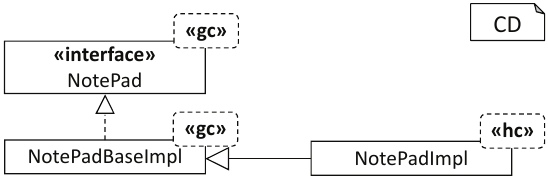
\epsfig{file = generation_gap.png, width = 7.5cm}}
		\caption{Generation Gap Muster f\"ur das NotePad-Beispiel\\ gc: generated code, hc: hand code}
		\label{fig:generation-gap-muster-fuer-das-notepad-beispiel}
	\end{figure}
	
	\section{Ergebnisse und Probleme}
	
	\subsection{Ergebnisse}
	
	Schlie\ss{}lich liegt nach der Arbeitsweise der gezielte Rest-Service vor. Dieser ist in der Lage die gew\"unschten Funktionalit\"aten anzubieten, die vorher abgesprochen waren. Die Daten sind durch die Datenbank und Speicherung der Daten auf einer AWS-S3-Instanz tats\"achlich persistent. Der Rest-Service kann ebenfalls entsprechende Antworten zur\"uckgeben:
	\begin{enumerate}
		\item 200 OK
		\item 400 Bad Request
		\item 403 Forbidden
		\item 404 Not Found
	\end{enumerate}
	
	\subsection{Probleme}
	
	W\"ahrend der Entwicklung ist das Team auf Schwierigkeiten gesto\ss{}en. Diese waren einerseits aufgrund der Verwendung eines Modellgetriebene-Software-Entwicklungswerkzeugs ausgel\"ost andererseits aufgrund der Datensicherheit bei der Nutzung vom AWS S3.
	
	\subsubsection{Un\"ubersichtlicher, generierter Code}
	
	Der von Swagger generierte Code ist an vielen Stellen un\"ubersichtlich. Der Code in den Controllern und Interfaces ist schwer zu verstehen  (Abbildung \ref{fig:quellcode-der-schnittstellen-getFile-und-editFile}). 
	
	\begin{figure}[ht]
		\centering
		{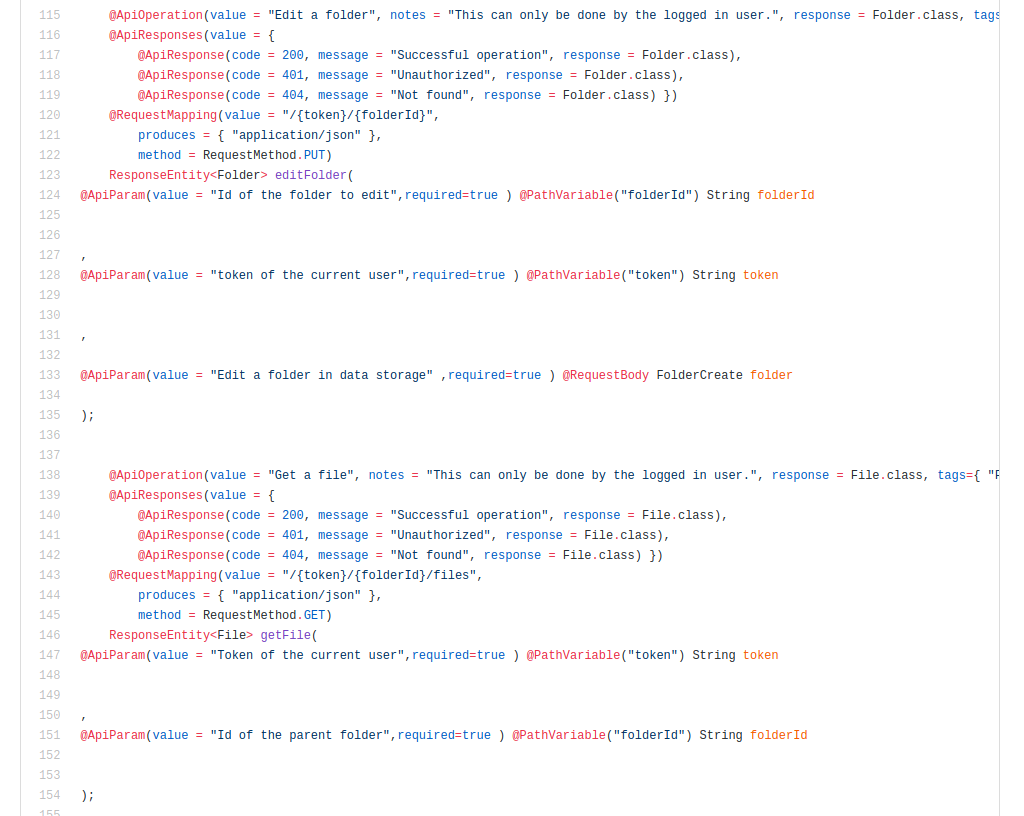
\epsfig{file = interfaces.png, width = 8cm}}
		\caption{Quellcode der Schnittstellen getFile und editFile}
		\label{fig:quellcode-der-schnittstellen-getFile-und-editFile}
	\end{figure}
	
	\subsubsection{Projektstruktur}
	
	Jeder Entwickler und jede Organisation k\"onnen ihre eigene Paketstruktur besitzen. Daher ist die von Swagger angebotene Paketstruktur immer auf dem ersten Blick ungew\"ohnlich (Abbildung \ref{fig:von-swagger-generierte-paketstruktur}). In dieser Abbildung ist das Paket io.swagger.service nicht von Swagger sondern von dem Entwicklungsteam generiert.
	
	\begin{figure}[ht]
		\centering
		{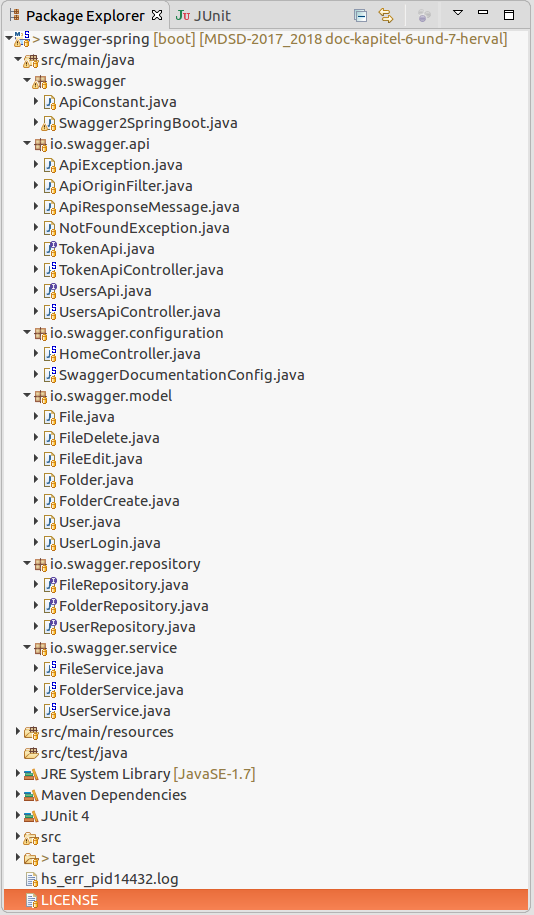
\epsfig{file = paketstruktur.png, width = 8cm}}
		\caption{Von Swagger generierte und vom Entwicklungsteam ver\"anderte Paketstruktur}
		\label{fig:von-swagger-generierte-paketstruktur}
	\end{figure}
	
	\subsubsection{Sicherheit}
	
	AWS bietet den S3-Dienst an, der erm\"oglicht Dateien auf eine Cloud zu speichern. Dies erfolgt per Quellcode mittels Access- und Secret-Keys. Damit das Team Transaktionen mit S3 w\"ahrend der Entwicklung durchf\"uren kann, soll es diese Schl\"ussel besitzen. Das Problem an der Stelle ist die Verteilung dieser Schl\"ussel. Diese kann zu b\"osen Zwecken verwendet werden und schlie\ss{}lich hohe Kosten f\"ur den offiziellen Besitzer verursachen. Au\ss{}erdem w\"aren sie \"offentlich f\"ur Hacker durch GitHub gewesen, da GitHub zur Versionsverwaltung verwendet wurde.
	Aus diesen Gr\"unden wurde ein Nexus-Repository entwickelt und geheim gehalten, damit diese Access- und Secret-Keys nicht verteilt werden. Dieses Repository stellt ein Object S3Transaction zur Verf\"ugung, das seinerseits Funktionen wie upload, rename und delete zur Verf\"ugung stellt. Die S3Transaction-Abh\"angigkeit ist anhand der folgenden Dependency aufzurufen:
	
	\begin{small}
		\begin{verbatim}
		<dependency>
		<groupId>
		com.mdsd-2017-2018.s3-transactions
		</groupId>
		<artifactId>
		s3-transactions
		</artifactId>
		<version>1.2.2</version>
		</dependency>
		\end{verbatim}
	\end{small}

	\subsubsection{Abst\"urtzen der EC2-Instanz}
	
	\vfill
	\bibliographystyle{apalike}
	{\small
		\bibliography{quellen}}
	
	\listoftables
	
	\listoffigures
\end{document}

